 \pstart \textso{Experim. VI.} Si aer in Tubo comprehensus \textit{ac} sit compressus vel dilatatus et \edtext{Mercurii \textit{ac} altitudo}{\lemma{et}\Afootnote{ \textit{ (1) }\ pondus\protect\index{Sachverzeichnis}{pondus|textit} \textit{ (2) }\ Mercurii \textit{ac} altitudo \textit{ L}}} minor est pollicibus dictis, tunc aer internus compressus Mercurium\protect\index{Sachverzeichnis}{mercurius} extrorsum pellet versus \textit{d} 
 [109 v\textsuperscript{o}] aere interno dilatato, externus eum introrsum pellet; utrumque fiet \edtext{eousque donec}{\lemma{fiet}\Afootnote{ \textit{ (1) }\ donec aer \textit{ (2) }\ eousque donec \textit{ L}}} \edtext{tensio}{\lemma{donec}\Afootnote{ \textit{ (1) }\ altitudo \textit{ (2) }\ tensio \textit{ L}}} compressiove\protect\index{Sachverzeichnis}{compressio} seu status aeris interni reductus sit ad statum aeris ordinarii seu externi. Nec referet quo in situ \edtext{perpendiculari, horizontali an}{\lemma{situ}\Afootnote{ \textit{ (1) }\ recto, an \textit{ (2) }\ perpendiculari, horizontali an \textit{ L}}} inclinato tubus statuatur. Ratio manifesta est ex dictis. Nec referet \edtext{etiam}{\lemma{}\Afootnote{etiam \textit{ erg.} \textit{ L}}} quanta sit altitudo Mercurii\protect\index{Sachverzeichnis}{mercurius}, dummodo sit minor pollicibus dictis, 27, (30) idem enim eveniet, sive \edtext{duorum triumve sive decem aut viginti pollicum}{\lemma{sive}\Afootnote{ \textit{ (1) }\ unius p \textit{ (2) }\ duorum [...] pollicum \textit{ L}}} sit Mercurius\protect\index{Sachverzeichnis}{mercurius}, dummodo \edtext{ad altitudinem}{\lemma{dummodo}\Afootnote{ \textit{ (1) }\ ille pol \textit{ (2) }\ altitudo \textit{ (3) }\ ad altitudinem \textit{ L}}} quae aeri externo aequiponderare potest, non ascendatur.
 \pend
%Zeitz auskommentiert%\rule[0cm]{0cm}{1cm}
%\begin{center}
%   
\includegraphics[width=0.2\textwidth]{images/37_3_109v1}\hspace{3cm}
%    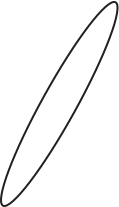
\includegraphics[width=0.1\textwidth]{images/37_3_109v2}\\ \textit{[Fig. 8, gestr.]}\hspace{22mm}\textit{[Fig. 9, gestr.]}\protect\rule[-1cm]{0cm}{1cm}\\
%   % \includegraphics[width=0.45\textwidth]{images/37_3_109v3}
%     %\includegraphics[width=0.45\textwidth]{images/37_3_109v4}\\
%     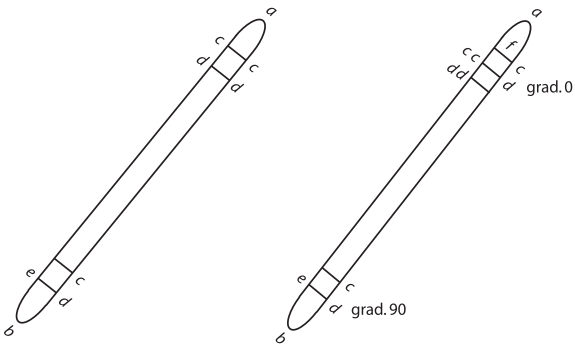
\includegraphics[width=0.9\textwidth]{images/37_3_109v3v4}\\
%    \textit{[Fig. 10, gestr.]}\hspace{4cm}\textit{[Fig. 11]}\rule[0cm]{3cm}{0cm}
%\end{center}
\clearpage
 \pstart \textso{Experim. VII.} \edtext{Ex dictis}{\lemma{\textso{Experim. VII.}}\Afootnote{ \textit{ (1) }\ Si \textit{ (2) }\ Si Tubus \textit{ (3) }\ Per Mercurium\protect\index{Sachverzeichnis}{mercurius|textit} \textit{ (4) }\ Ex dictis \textit{ L}}} sequitur etiam praxis construendi \textso{Instrumenti inclinationum,}\protect\index{Sachverzeichnis}{instrumentum!inclinationum} cujus ope scilicet sine \edtext{mensuratione}{\lemma{sine}\Afootnote{ \textit{ (1) }\ calculo ac dim \textit{ (2) }\  mensuratione \textit{ L}}} ex aspectu disci possit, quis sit angulus inclinationis; \edtext{et quanta inclinati vis si recto \edlabel{comp109v1}comparetur.}{\lemma{et}\Afootnote{ \textit{ (1) }\ quis \textit{ (2) }\ quae vis inclinati in compara \textit{ (3) }\ quanta [...] comparetur. \textit{ L}}} \edtext{\edlabel{comp109v2}Sumatur Tubus \textit{ab} implendus aere dilatato, et utrinque claudendus}{\lemma{comparetur.}\xxref{comp109v1}{comp109v2}\Afootnote{ \textit{ (1) }\ Communis \textit{ (2) }\ Baroscopium\protect\index{Sachverzeichnis}{baroscopium|textit} hoc tantum habet \textit{ (3) }\ Sumatur Tu \textit{ (4) }\ Inseratur Mercurius\protect\index{Sachverzeichnis}{mercurius|textit} in Tubum utrumque clausum \textit{ (5) }\ Sumatur [...] claudendus \textit{ L}}} quod ita commode fiet, si ad lampadem summe calefiat, statimque claudatur, dummodo ea sit vitri\protect\index{Sachverzeichnis}{vitrum} fortitudo ut ab aeris externi compressione\protect\index{Sachverzeichnis}{compressio} non rumpatur. Si rupturae metus est, aer non nimis calefiat. Potest Instrumentum 
% \begin{wrapfigure}{l}{0.1\textwidth}                    
        %        
\includegraphics[width=0.1\textwidth]{images/37_3_109v1}
                        %\caption{Bildbeschreibung}
    %                    \end{wrapfigure}
                        %@ @ @ Dies ist eine Abstandszeile - fuer den Fall, dass mehrere figures hintereinander kommen, ohne dass dazwischen laengerer Text steht. Dies kann zu einer Fahlermeldung fuehren. @ @ @ \\
            %         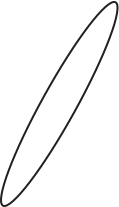
\includegraphics[width=0.1\textwidth]{images/37_3_109v2}% \begin{wrapfigure}{l}{0.4\textwidth}                    
                %\includegraphics[width=0.4\textwidth]{../images/Propositio+experimentorum+novorum/LH037%2C03_109v/files/100202.png}
                        %\caption{Bildbeschreibung}
                        %\end{wrapfigure}
                        %@ @ @ Dies ist eine Abstandszeile - fuer den Fall, dass mehrere figures hintereinander kommen, ohne dass dazwischen laengerer Text steht. Dies kann zu einer Fahlermeldung fuehren. @ @ @ \\
                %     \includegraphics[width=0.4\textwidth]{images/37_3_109v3}% \begin{wrapfigure}{l}{0.4\textwidth}                    
                %\includegraphics[width=0.4\textwidth]{../images/Propositio+experimentorum+novorum/LH037%2C03_109v/files/100204.png}
                        %\caption{Bildbeschreibung}
                        %\end{wrapfigure}
                        %@ @ @ Dies ist eine Abstandszeile - fuer den Fall, dass mehrere figures hintereinander kommen, ohne dass dazwischen laengerer Text steht. Dies kann zu einer Fahlermeldung fuehren. @ @ @ \\
                    % \includegraphics[width=0.4\textwidth]{images/37_3_109v4}% \begin{wrapfigure}{l}{0.4\textwidth}                    
                %\includegraphics[width=0.4\textwidth]{../images/Propositio+experimentorum+novorum/LH037%2C03_109v/files/100206.png}
                        %\caption{Bildbeschreibung}
                        %\end{wrapfigure}
                        %@ @ @ Dies ist eine Abstandszeile - fuer den Fall, dass mehrere figures hintereinander kommen, ohne dass dazwischen laengerer Text steht. Dies kann zu einer Fahlermeldung fuehren. @ @ @ \\
                 %   \edtext{}{\lemma{}\Bfootnote{Zeichnung \lbrack fig. n \rbrack - \lbrack fig. n+1 \rbrack gestrichen.}} % \begin{wrapfigure}{l}{0.4\textwidth}                    
                %\includegraphics[width=0.4\textwidth]{../images/Propositio+experimentorum+novorum/LH037%2C03_109v/files/100211.png}
                        %\caption{Bildbeschreibung}
                        %\end{wrapfigure}
                        %@ @ @ Dies ist eine Abstandszeile - fuer den Fall, dass mehrere figures hintereinander kommen, ohne dass dazwischen laengerer Text steht. Dies kann zu einer Fahlermeldung fuehren. @ @ @ \\
                     fieri aere non dilatato, sed ita plus mercurii\protect\index{Sachverzeichnis}{mercurius} adhibendum est, quod tubi usum reddit incommodiorem. Tubus quanto longior est, tanto accuratius subdividi potest, tantoque plus Mercurii\protect\index{Sachverzeichnis}{mercurius} est adhibendum, etsi \edtext{Instrumentum ita fiat minus portabile}{\lemma{etsi}\Afootnote{ \textit{ (1) }\ usus aeque commodus non \textit{ (2) }\ Instrumentum ita fiat minus portabile \textit{ L}}}. Mercurius\protect\index{Sachverzeichnis}{mercurius} Instrumento inserendus est antequam claudatur. Instrumento \edtext{perpendiculariter}{\lemma{}\Afootnote{perpendiculariter \textit{ erg.} \textit{ L}}} erecto, Mercurius\protect\index{Sachverzeichnis}{mercurius} \edtext{\textit{cd} in summitate Tubi \textit{a} positus pondere sui descensus aerem subjectum, comprimet}{\lemma{Mercurius}\Afootnote{ \textit{ (1) }\ id pondere suo comprimet \textit{ (2) }\   \textbar\ \textit{cd} \textit{ erg.}~\textbar\ in [...] comprimet \textit{ L}}}, qui cum parum resistat, est enim dilatatus ac proinde facile fert compressionem\protect\index{Sachverzeichnis}{compressio} \edtext{ut in Recipiente Magdeburgico\protect\index{Sachverzeichnis}{Recipiens!Magdeburgicum} exhausto aquam Mercuriumque\protect\index{Sachverzeichnis}{mercurius} si aere purgato non sint ex Tubo descendere videmus, quippe aeris dilatati pressione\protect\index{Sachverzeichnis}{pressio!aeris} eum minus sustinente}{\lemma{}\Afootnote{ut in Recipiente Magdeburgico\protect\index{Sachverzeichnis}{Recipiens!Magdeburgicum}   \textbar\ exhausto \textit{ erg.}\ \textbar\  aquam Mercuriumque\protect\index{Sachverzeichnis}{mercurius}  \textbar\ si aere purgato non sint \textit{ erg.}\ \textbar\  ex [...] sustinente \textit{ erg.} \textit{ L}}}; ideo Mercurius\protect\index{Sachverzeichnis}{mercurius} pene descendet ad fundum usque \textit{b} \edtext{seu usque ad \textit{e}.}{\lemma{}\Afootnote{seu usque ad \textit{e}. \textit{ erg.} \textit{ L}}} Notetur \edtext{in Tubo quousque}{\lemma{}\Afootnote{in Tubo quousque \textit{ erg.} \textit{ L}}} maximus Mercurii\protect\index{Sachverzeichnis}{mercurius} descensus pervenit is repraesentat situm machinae perpendicularem; notetur descensus ejus minimus, seu locus summus, \edtext{in quem redit Tubo Horizontaliter posito,}{\lemma{summus,}\Afootnote{ \textit{ (1) }\ in qu \textit{ (2) }\ ex quo descendere incipit. Is idem est cum altitudine  \textit{(a)}\ Mercurii\protect\index{Sachverzeichnis}{mercurius|textit} \textit{(b)}\ Tubi \textit{a}. Notetur \textit{ (3) }\ seu \textit{ (4) }\ in [...] posito, \textit{ L}}} non scilicet perveniet usque ad \textit{a} etsi primo delapsus sit ex \textit{a} quia cum \edtext{aere}{\lemma{}\Afootnote{aere \textit{ erg.} \textit{ L}}} purgatus non fuerit, ideo ut descendere possit aerem ex \edtext{corpore suo}{\lemma{ex}\Afootnote{ \textit{ (1) }\ substantia sua \textit{ (2) }\ corpore suo \textit{ L}}} exprimet, dilatabitque, qui non redibit facile in Mercurium\protect\index{Sachverzeichnis}{mercurius}, ac proinde \edtext{aer hoc Mercurio horizontaliter posito non dilatatus neque compressus implebit spatium \textit{af} inter Mercurium \textit{cc-dd} et summitatem \textit{a}.}{\lemma{proinde}\Afootnote{ \textit{ (1) }\ Mercurius\protect\index{Sachverzeichnis}{mercurius|textit} non ascendet usque ad spatium hoc aere plenum semper \textit{ (2) }\ aer [...] compressus \textit{(a)}\ imprimet \textit{(b)}\ implebit [...] \textit{a}. \textit{ L}}} Nota ergo Tubi Horizontalis erit \textit{f}. Adhibito \edtext{jam}{\lemma{}\Afootnote{jam \textit{ erg.} \textit{ L}}} quadrante 
                     [110~r\textsuperscript{o}] omnes anguli inclinationis\protect\index{Sachverzeichnis}{inclinatio} observentur, et quis in quoque Mercurii\protect\index{Sachverzeichnis}{mercurius} sit ascensus notetur. Hoc facto quoties \edtext{indagare placet corporis alicujus inclinationem. Locetur Instrumentum in situ ei parallelo quod dioptris adhibitis facile fiet si res est remota, et simplici applicatione si propinqua; statim}{\lemma{quoties}\Afootnote{ \textit{ (1) }\ Instrumentum tecum habebis aspectus  \textit{(a)}\ statim sine \textit{(b)}\ et \textit{ (2) }\ indagare placet  \textit{(a)}\ situm \textit{(b)}\ corporis [...] statim \textit{ L}}} tibi angulum Mercurius\protect\index{Sachverzeichnis}{mercurius} dabit. Hac arte \edtext{et}{\lemma{}\Afootnote{et \textit{ erg.} \textit{ L}}} horizontem et perpendiculum et elevationem stellae\protect\index{Sachverzeichnis}{elevatio!stellae} cujusdam alteriusve corporis altitudinem, quotiescunque summa exactitudine opus non est, facile \edtext{habebimus}{\lemma{facile}\Afootnote{ \textit{ (1) }\ sumemus \textit{ (2) }\ habebimus \textit{ L}}}\footnote{\textit{Nebenrechnung rechte Spalte:}\\
\protect\begin{tabular}{l}
\hspace{5.5pt}36\\
\hspace{11pt}600\\
$\overline{21600}$
\protect\end{tabular}}. Quanquam si in minuta usque \edtext{prima}{\lemma{}\Afootnote{prima \textit{ erg.} \textit{ L}}} dividatur \edtext{quod difficile non est}{\lemma{}\Afootnote{quod difficile non est \textit{ erg.} \textit{ L}}}, ad rem nauticam et Geometriam practicam sufficiat\edtext{. Ita}{\lemma{sufficiat}\Afootnote{ \textit{ (1) }\ ; rectius pro \textit{ (2) }\ . Ita \textit{ L}}} in uno instrumento habebimus compendium multorum. Poterit Tubis applicari, et Dioptris, et Mensulis Geometricis. Perpendiculum vibrationibus suis continuis valde impedit, quominus linea perpendicularis exacte sumatur. Linea Horizontalis sumenda est aut sumta jam perpendiculari, alia ad angulos ad tam rectos ducta, aut sine perpendiculari, ope liquoris\protect\index{Sachverzeichnis}{liquor}, cujus superficies est horizontalis. Sed cum ipsa liquorum\protect\index{Sachverzeichnis}{liquor} superficies non sit perfecte aequalis, \edtext{et}{\lemma{aequalis,}\Afootnote{ \textit{ (1) }\ se \textit{ (2) }\ et \textit{ L}}} modo in medio modo in extremo altior, hinc nova erroris occasio, cui Instrumento isto infallibiliter \edtext{occurretur. Hactenus usus Instrumenti ad}{\lemma{occurretur.}\Afootnote{ \textit{ (1) }\ Et hic est potissimum usus Instrumenti ad \textit{ (2) }\ Hactenus usus Instrumenti ad \textit{ L}}} inveniendas \edtext{lineas Horizontalem perpendicularem, aut mediae gradum seu Inclinationem}{\lemma{inveniendas}\Afootnote{ \textit{ (1) }\ Inclinationes\protect\index{Sachverzeichnis}{inclinatio|textit}, id est \textit{ (2) }\ lineas [...] Inclinationem \textit{ L}}}, in re mensoria, \edtext{Geographica,}{\lemma{Geographica,}\Afootnote{\textbar\ Astronomica \textit{ gestr.}\ \textbar\   Nautica \textit{ erg.} \textit{ L}}} Nautica, Hydrostatica, Architectura civili militarique maximus. Restant alii duo, primum \textso{Mechanicus,} deinde quod mireris \textso{Geometricus.} Mechanicus est data inclinatione\protect\index{Sachverzeichnis}{inclinatio} invenire \edtext{vim ponderis}{\lemma{invenire}\Afootnote{ \textit{ (1) }\ pondus\protect\index{Sachverzeichnis}{pondus|textit} \textit{ (2) }\ vim ponderis \textit{ L}}} in plano inclinato. Ea erit in ea ratione \edtext{ad vim ponderis perpendicularis in qua est altitudo descensus inclinationis datae, ad altitudinem descensus perpendicularis.}{\lemma{ratione}\Afootnote{ \textit{ (1) }\ in qua est altitudo descensus hori \textit{ (2) }\ ad [...] altitudo \textit{(a)}\ descensus anguli dati \textit{(b)}\ descensus [...] perpendicularis. \textit{ L}}} \edtext{Eodem modo et ictus\protect\index{Sachverzeichnis}{ictus} obliqui mensurabuntur.}{\lemma{}\Afootnote{Eodem [...] mensurabuntur. \textit{ erg.} \textit{ L}}} Usus \textso{Geometricus} est, habere instrumentum cujus ope inveniatur Angulo dato, ratio secantis ad radium, seu duorum secantium inter se, sunt enim secantes seu radius et secans, (radius enim potest dici secantium primus seu minimus) ut altitudines descensus in instrumento reciproce. Ecce instrumentum simplicissimum maximi usus.
\pend